\section{Mở đầu}

\subsection{Bối cảnh và mục tiêu}
Hệ thống chính của đồ án dự báo chất lượng nước và phân loại mức độ phù hợp nuôi trồng (con hàu, cá giò) dựa trên dữ liệu quan trắc theo quý. Giai đoạn cuối, dự án được bổ sung nguồn \textbf{dữ liệu thời gian thực GreenLab} --- hệ thống quan trắc môi trường IoT của Đại Học Thái Bình.

Mục tiêu của module thực nghiệm:
\begin{enumerate}[nosep]
  \item \textbf{Giám sát:} so các chỉ số đo được với ngưỡng QCVN 10:2023/BTNMT (cột B1 --- nuôi trồng thủy sản).
  \item \textbf{Phân loại:} từ 5 chỉ số cảm biến, suy ra đủ bộ chỉ số đầu vào cho mô hình phân loại phù hợp.
\end{enumerate}

Module được xây dựng \emph{độc lập} dưới \texttt{lab/realtime\_greenlab/}, không phụ thuộc webapp, import trực tiếp logic từ \texttt{src/} --- theo tiền lệ các thực nghiệm forecast trước đó.

\subsection{Nguồn dữ liệu GreenLab}
Dữ liệu lưu trên MongoDB Atlas (collection \texttt{quan\_trac}, document type \texttt{greenlab\_latest\_snapshot}). Hệ thống có \textbf{4 trạm}, mỗi trạm 5 cảm biến cố định (Bảng~\ref{tab:stations}).

\begin{table}[h]
\centering\small
\caption{Bốn trạm quan trắc GreenLab (nguồn: \texttt{stations.yaml}).}
\label{tab:stations}
\begin{tabular}{llll}
\toprule
\textbf{Serial} & \textbf{Vị trí} & \textbf{Loại nước} & \textbf{Trạng thái} \\
\midrule
06M26042804 & Làng bè Cát Bà, Hải Phòng & ven biển & \textbf{có dữ liệu} (cobia) \\
06M26042803 & Làng bè Vân Đồn, Quảng Ninh & ven biển & chưa kích hoạt (oyster) \\
06M26042802 & Hưng Yên & nội địa & ngoài phạm vi \\
06M26042801 & Hưng Yên & nội địa & ngoài phạm vi \\
\bottomrule
\end{tabular}
\end{table}

Tại thời điểm phân tích, chỉ trạm Cát Bà (\texttt{06M26042804}) có dữ liệu. Năm chỉ số đo: COD, NH4, pH, nhiệt độ (Temp), TSS.

\subsection{Mô tả và trực quan dữ liệu}
\textbf{Độ phủ.} \textbf{15.475 bản ghi} trải \textbf{23 ngày} (29/05--20/06/2026), một trạm. Tần suất ban đầu $\sim$3--5 phút/lần ($\approx$288 reading/ngày), \emph{tăng vọt lên 1 phút/lần} ($\approx$1.440/ngày) từ 12/06 (Hình~\ref{fig:coverage}) --- nửa sau dữ liệu dày hơn nửa đầu $\sim$5 lần.

\begin{figure}[h]
\centering
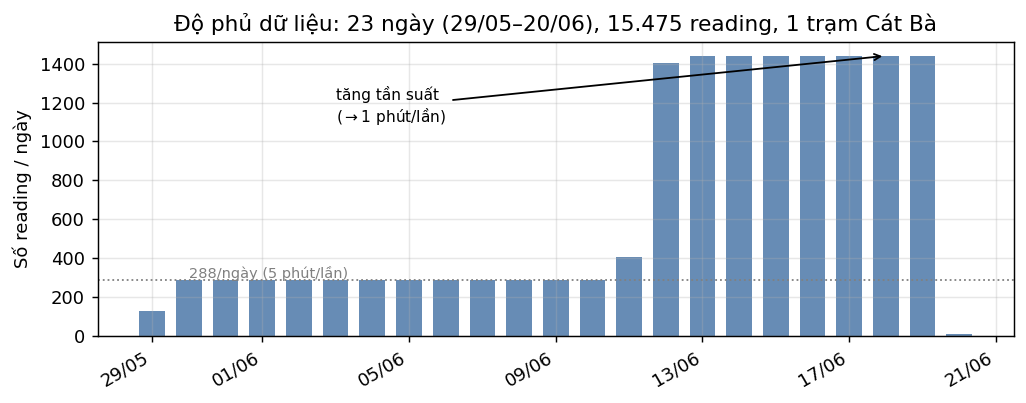
\includegraphics[width=0.92\linewidth]{../figures/data_coverage.png}
\caption{Số reading mỗi ngày. Bước nhảy 12/06 phản ánh thay đổi cấu hình tần suất phía vận hành, không phải sự kiện môi trường.}
\label{fig:coverage}
\end{figure}

\textbf{Thống kê mô tả} (Bảng~\ref{tab:desc}) đã hé lộ bất thường ngay từ trung vị: COD trung vị $=558{,}8$ trùng đúng giá trị lớn nhất (dấu hiệu kẹt trần), NH4 thô hàng trăm lần ngưỡng QCVN.

\begin{table}[h]
\centering\small
\caption{Thống kê mô tả 5 cảm biến (15.475 reading).}
\label{tab:desc}
\begin{tabular}{lrrrrr}
\toprule
\textbf{Chỉ số} & \textbf{min} & \textbf{trung vị} & \textbf{max} & \textbf{độ lệch chuẩn} & \textbf{ngưỡng QCVN B1} \\
\midrule
COD (mg/L)  & 6{,}4  & \textbf{558{,}8} & 558{,}8 & 204{,}0 & 10 \\
NH4 (thô)   & 77{,}6 & 114{,}6 & 160{,}3 & 16{,}7  & --- (xem NH3) \\
pH          & 7{,}78 & 7{,}98  & 8{,}41  & 0{,}10  & 6{,}5--8{,}5 \\
Temp (°C)   & 26{,}6 & 30{,}2  & 33{,}0  & 0{,}76  & --- \\
TSS (mg/L)  & 1{,}1  & 47{,}1  & 237{,}9 & 24{,}0  & 50 \\
\bottomrule
\end{tabular}
\end{table}

\textbf{Phân phối giá trị} (Hình~\ref{fig:dist}) làm rõ hình dạng: COD \emph{lưỡng đỉnh} --- một cụm nhỏ quanh 10 (giai đoạn đầu) và một khối lớn dồn ở trần 558{,}8; pH/Temp tập trung chặt trong dải hợp lý; TSS lệch phải mạnh (42\% reading vượt 50). Diễn biến theo thời gian của bốn cảm biến còn sống ở Hình~\ref{fig:panel}.

\begin{figure}[h]
\centering
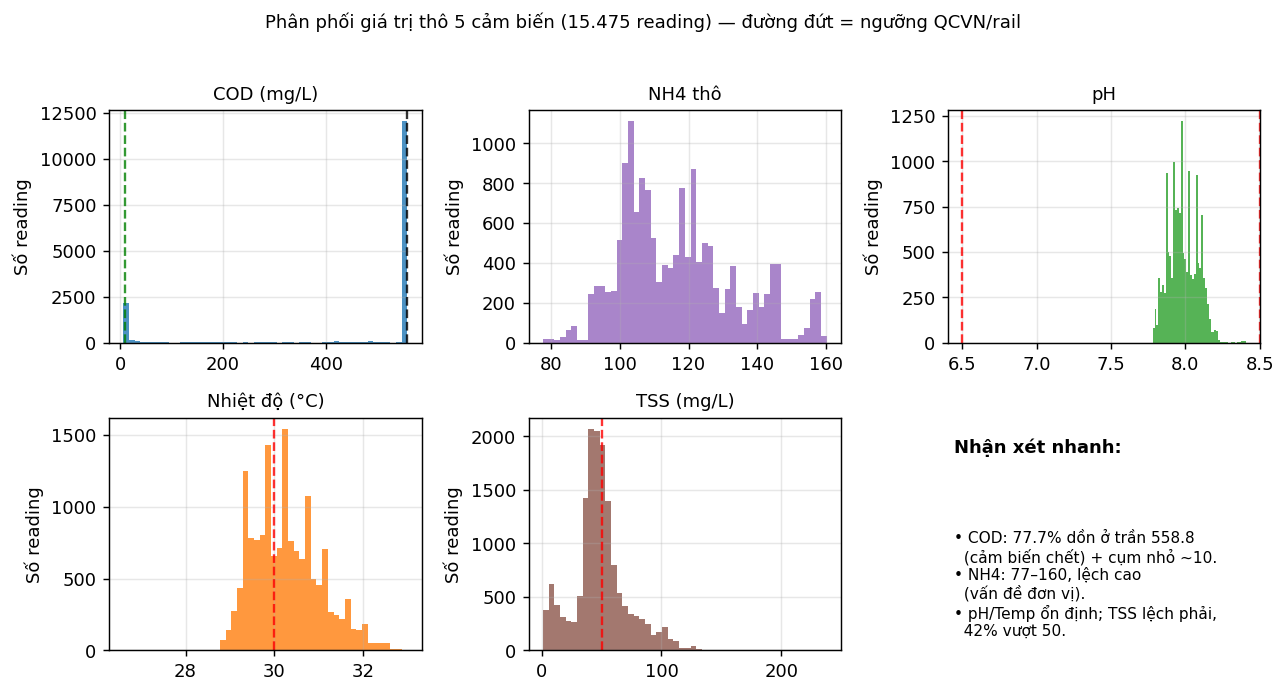
\includegraphics[width=\linewidth]{../figures/value_dist.png}
\caption{Histogram giá trị thô 5 cảm biến. COD dồn ở trần 558{,}8 (cảm biến chết); NH4 lệch cao bất thường; pH/Temp ổn định; TSS lệch phải.}
\label{fig:dist}
\end{figure}

\begin{figure}[h]
\centering
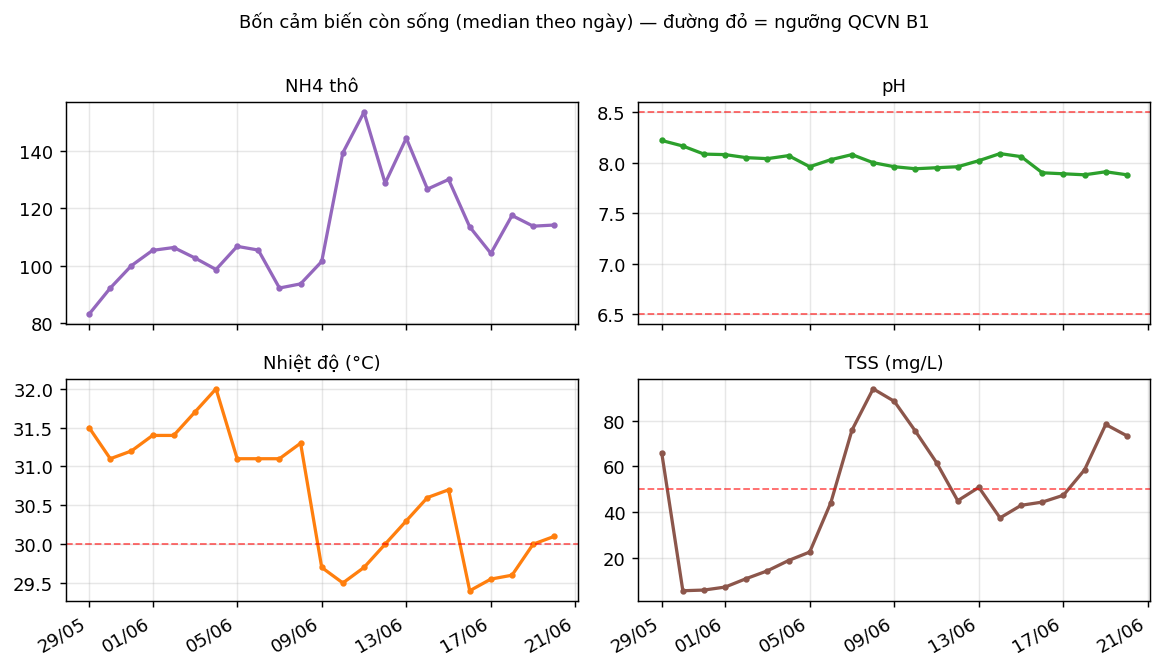
\includegraphics[width=\linewidth]{../figures/sensor_panel.png}
\caption{Diễn biến median theo ngày của bốn cảm biến còn hoạt động. pH, nhiệt độ, TSS dao động hợp lý; NH4 thô ở mức cao (vấn đề đơn vị).}
\label{fig:panel}
\end{figure}

\subsection{Vấn đề phát hiện trong dữ liệu thu thập}
Phân tích trên bộc lộ ba vấn đề cần xử lý trước khi dùng (chi tiết ở Mục~\ref{sec:phuongphap}):
\begin{enumerate}[nosep]
  \item \textbf{Cảm biến COD đã chết} --- 77{,}7\% reading kẹt cứng ở trần 558{,}8 mg/L (phương sai 0), không phải ô nhiễm thật mà là bão hòa cảm biến.
  \item \textbf{Đơn vị NH4 chưa xác định} --- giá trị thô 77--160; nếu là mg/L thì vô lý cho nước nuôi trồng. Thêm nữa cảm biến đo NH4$^+$ trong khi QCVN đánh giá NH3.
  \item \textbf{TSS và nhiệt độ thường xuyên vượt ngưỡng} --- TSS$>$50: 42\% reading; Temp$>$30: 57\% --- đây là tín hiệu thật, cần phản ánh đúng ở phần giám sát.
\end{enumerate}

\subsection{Vấn đề cốt lõi: thiếu chỉ số}
\label{sec:thieuchiso}
Mô hình phân loại cần \textbf{19 chỉ số} (cá giò Hải Phòng) hoặc \textbf{20 chỉ số} (hàu Quảng Ninh); cảm biến chỉ cấp 5. Để lấp khoảng trống, các chỉ số được \textbf{xử lý theo nhóm} (cascade 4 tầng nguồn gốc, Bảng~\ref{tab:gap}) --- ưu tiên đo thật, rồi hóa học, rồi ML, cuối cùng mới trung vị.

\begin{table}[h]
\centering\small
\caption{Cascade 4 tầng: nguồn gốc các chỉ số đưa vào phân loại (mức tin cậy giảm dần từ trên xuống).}
\label{tab:gap}
\begin{tabular}{lll}
\toprule
\textbf{Tầng (nhóm)} & \textbf{Chỉ số / cách lấy} & \textbf{Độ tin} \\
\midrule
1. Đo trực tiếp & pH, nhiệt độ, TSS (+ COD khi QC đạt) & cao nhất \\
2. Suy ra (hóa học) & NH3 (từ NH4 + pH + Temp qua Emerson) & cao \\
3. Nội suy (ML) & DO, BOD5, Transparency, Alkalinity, PO4 & tùy $R^2$ \\
4. Mặc định (trung vị) & Salinity, kim loại nặng, Coliform, H2S, \dots & thấp nhất \\
\bottomrule
\end{tabular}
\end{table}

DO và độ muối là hai chỉ số quan trọng nhất (trọng số 1 và 2 cho cả hàu lẫn cá giò) nhưng đều không đo được trực tiếp --- đây là gốc rễ của các hạn chế nêu ở Mục~\ref{sec:thaoluan}.
